\chapter{Introduction}

\section {Motivation}

Single core performance in CPUs has stalled for the last 10 years as processor manufacturers focus on multi-core systems in order to increase performance \cite{procspeed2}. Unfortunately, most of the existing software can not take advantage of the increasing processing speed, because they operate sequentially. Since replacing hardware will not have as much of an impact as it had in the past \cite{procspeed}, scaling existing systems to meet new requirements becomes more difficult.

Parallelizing software is a daunting proposition as software architectures have a purely sequential design. The programmers involved need to identify parts of their application that consume the most processing time and decide whether it is actually expedient to parallelize them.

This thesis presents a framework with two tools developed using Intel Pin \cite{pin} that use dynamic binary instrumentation to obtain information about a application. In order to utilize this data multiple visualizations were developed that help the user in determining which parts of an application can be parallelized. The framework can be easily extended to gather more information that can be displayed in tailored visualizations.

The framework is based on the concept of tagging sections of a programs source code. This is done interactively or can be inferred automatically by another tool. The tags are then applied to the program when it is instrumented. Changes to the source code of the applications are not required for this tool to function because tags are stored in a separate configuration file. This makes instrumenting a painless process on complex systems or when dealing with convoluted build processes.

In order to illustrate the usefulness of tools in the analysis of existing software we will present a simple example program in Figure \ref{cap1:emsim:seq}, which needs to be parallelized. The file is part of a simulator for the UEFA European Championship that was implemented sequentially.

\begin{figure}
	\begin{center}
		\inputminted[linenos, fontsize=\scriptsize]{c}{emsim_seq.c}
	\end{center}
	\caption{\texttt{emsim\_seq.c}: EM Simulator sequential implementation}
	\label{cap1:emsim:seq}
\end{figure}

Profiling indicates that the loops present in this code take up almost all the execution time as can be seen in Figure \ref{cap1:emsim:profile}. Loops in have a high potential for parallelism, but it can only be achieved if there are no dependencies between the iterations. Unfortunately it is difficult to analyze such dependencies. For example, the pointer arithmetic present in the loop starting in line 12 makes source code inspection very challenging, without understanding the logic behind the implementation it becomes impossible. Generally, it is difficult to grasp the dependencies without a thorough understanding of the application and careful analysis. 

\begin{figure}[!ht]
	\centering
	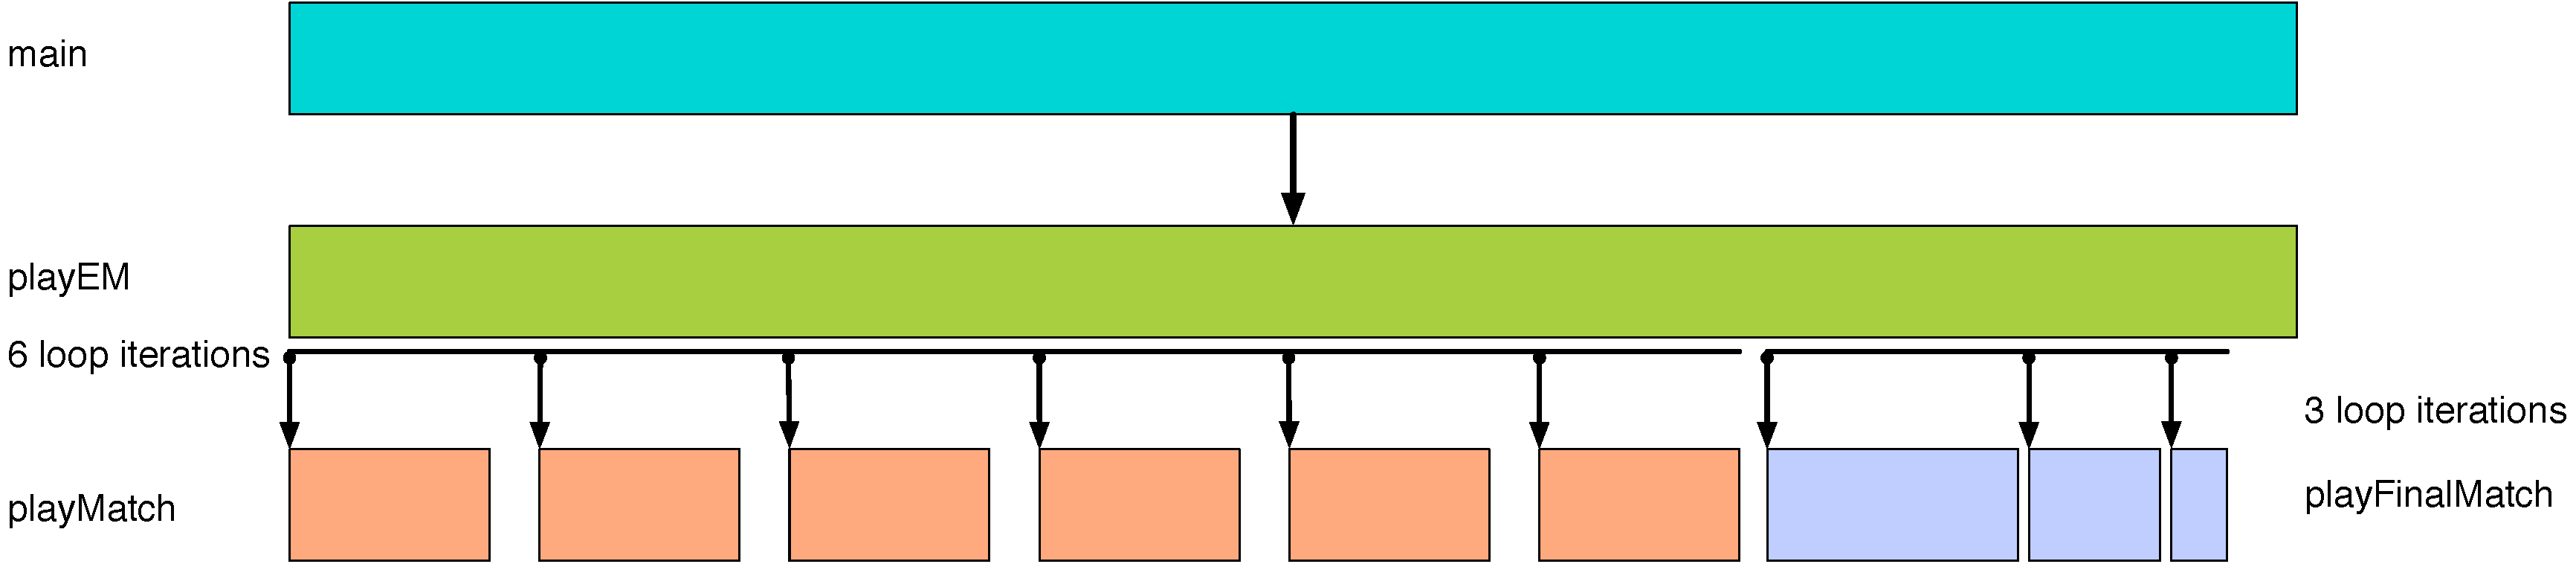
\includegraphics[width=0.8\textwidth]{emsimprofile}
	\caption{Profile view of the execution the code using Parceive}
	\label{cap1:emsim:profile}
\end{figure}

One of our visualizations is able to simulate the speed up when running sections of code in parallel to each other and to show the memory dependencies between the sections. Visualizations of loops on lines 12 and 30 in Figures \ref{cap1:emsim:sections1} and \ref{cap1:emsim:sections2} respectively show the possible speedup when running on a machine with 4 threads and more importantly the actual conflicts that the user must resolve in order to maintain correctness. The loop on line 12 can be easily modified to run in separate threads, even though all iterations work on the same arrays, since iterations works on distinct elements.

\begin{figure}[!ht]
	\centering
	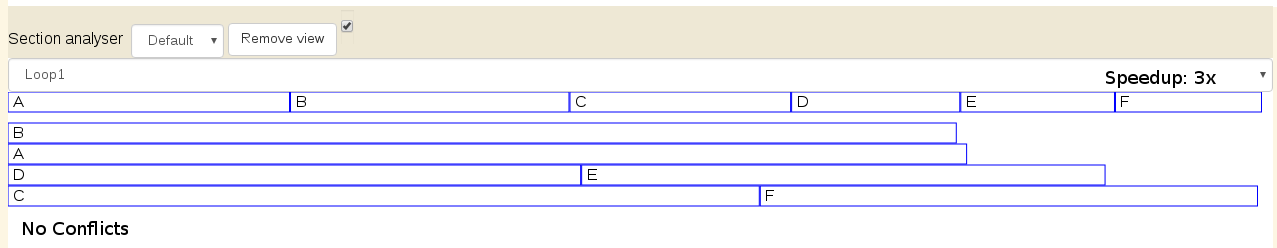
\includegraphics[width=0.8\textwidth]{loop1section}
	\caption{Section view of the loop on line 12 in Figure \ref{cap1:emsim:seq}}
	\label{cap1:emsim:sections1}
\end{figure}

\begin{figure}[!ht]
	\centering
	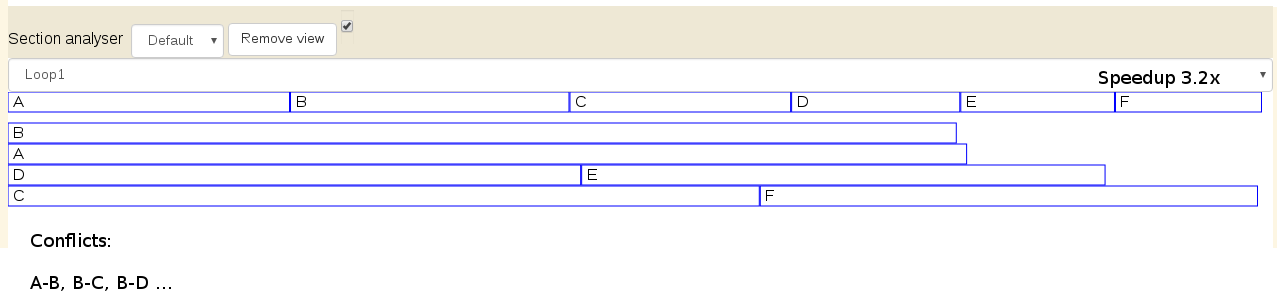
\includegraphics[width=0.8\textwidth]{loop2section}
	\caption{Section view of the loop on line 30 in Figure \ref{cap1:emsim:seq}}
	\label{cap1:emsim:sections2}
\end{figure}

As can be seen in these examples, information about the program can be gained by our tools. Profiling is a well known method of finding performance hot-spots in applications. In this thesis we propose tools that can help determine the potential for parallelization of these sections of code by simulating their parallel execution. This gives the user information about the possible speedup and the conflicts that require the code to remain sequential.

\section{Parceive}

Parceive \cite{parceive} is a tracing-based tool for parallelizing existing sequential software. It focuses on high-level architecture analysis, but also gathers fine-grained memory accesses and call information. We describe this tool in mode detail in Section \ref{cap2:parceive}

\section {Contribution}

This thesis presents a framework for gathering information about applications using dynamic binary instrumentation and tagging of the source code. Two analyses have been developed to help users when parallelizing existing applications, but more can be easily developed.

The first is section analysis, which simulates running parts of the source code in parallel. In Figures \ref{cap1:emsim:sections1} and \ref{cap1:emsim:sections2} the loops are tagged as sections and each iteration starts a new task. The visualization presents the possible performance benefit and conflicts when running the tasks within a section in parallel.

Our framework can also perform pipeline analysis to cover a different use case. Pipeline parallelism can be be applied to some loops, despite the fact that iterations can not be run in parallel to each other. This approach splits each iteration into stages and different stages from different iterations can be run parallel to each other. As a simple example we consider file processing, where data is read, processed and written to another file. Individual iterations can not be run in parallel, but the io operations and the processing can be seen in Figure \ref{cap1:pipeline}. In Chapter §2 we will present a more concrete example, bzip compression.

\begin{figure}[!ht]
	\centering
	\begin{tabular}{ l | l | l | l | l}
		R & P & W & & \\
		\hline
		R &  & P & W & \\
		\hline
		R &  & & P & W \\
	\end{tabular}
	\caption{Pipeline, R - read, P - proecess, W - write}
	\label{cap1:pipeline}
\end{figure}

\section {Example}

To better illustrate the use of our tools we will go trough a simple example that will be parallelized. The relevant code is shown in Figure \ref{cap1:emsim:seq}.

\subsection {Static analysis}

The first step a user must perform is the static analysis. This extracts all locations in the source code where a tag can be inserted. The application itself is executed in order to analyze all dynamic libraries that it uses.

\subsection{Execution}

\begin{lstlisting}[style=BashInputStyle]
pin.sh -t libpintool\_static.so -db emsim.db -filter filter.yaml \
  -- emsim_seq
\end{lstlisting}

This command starts pin and loads \texttt{libpintool\_static.so} as a tool. The result is saved in the \textbf{emsim.db} database. The command to start the application that is being instrumented follows \texttt{--}. The filter in Figure \ref{cap1:filter} is used to reduce the amount of work needed to be performed

\begin{figure}
	\begin{center}
		\begin{minted}{yaml}
image:
  exclude:
    - /lib64/*
file:
  exclude:
    - /usr/include
    - Unknown
    - sqlite.c
function:
  exclude:
  - _GLOBAL__*
  - __static_initialization_and_destruction_0
		\end{minted}
	\end{center}
	\caption{\texttt{filter.yaml} example}
	\label{cap1:filter}
\end{figure}

On systems with a more recent kernel it is necessary to supply Pin with the \texttt{-ifeellucky} to avoid some ineffective version checks.

\subsection {Tagging the code}

First the database must be copied to the import folder of \texttt{parceive-ui} and processed:

\begin{lstlisting}[style=BashInputStyle]
gulp db
\end{lstlisting}

Then the UI can be started:

\begin{lstlisting}[style=BashInputStyle]
gulp server
\end{lstlisting}

Figure \ref{cap1:tagview} shows the UI to tag code. Using this interface 2 \textbf{Tags} are defined, \textit{Section 1} and \textit{Section 1 Task}. Three \textbf{TagInstructions} are then defined to delimit the sections of code.

\textit{Section 1} has a \texttt{Start} at line 11 and a \texttt{Stop} at line 22. This encompasses the entire loop.  \textit{Section 1 Task} has only a \texttt{Start} at line 14. Each iteration a new task is started and the old one is automatically closed. Figure \ref{cap1:source} shows the generated \texttt{source.yaml}.

\begin{figure}[!ht]
	\centering
	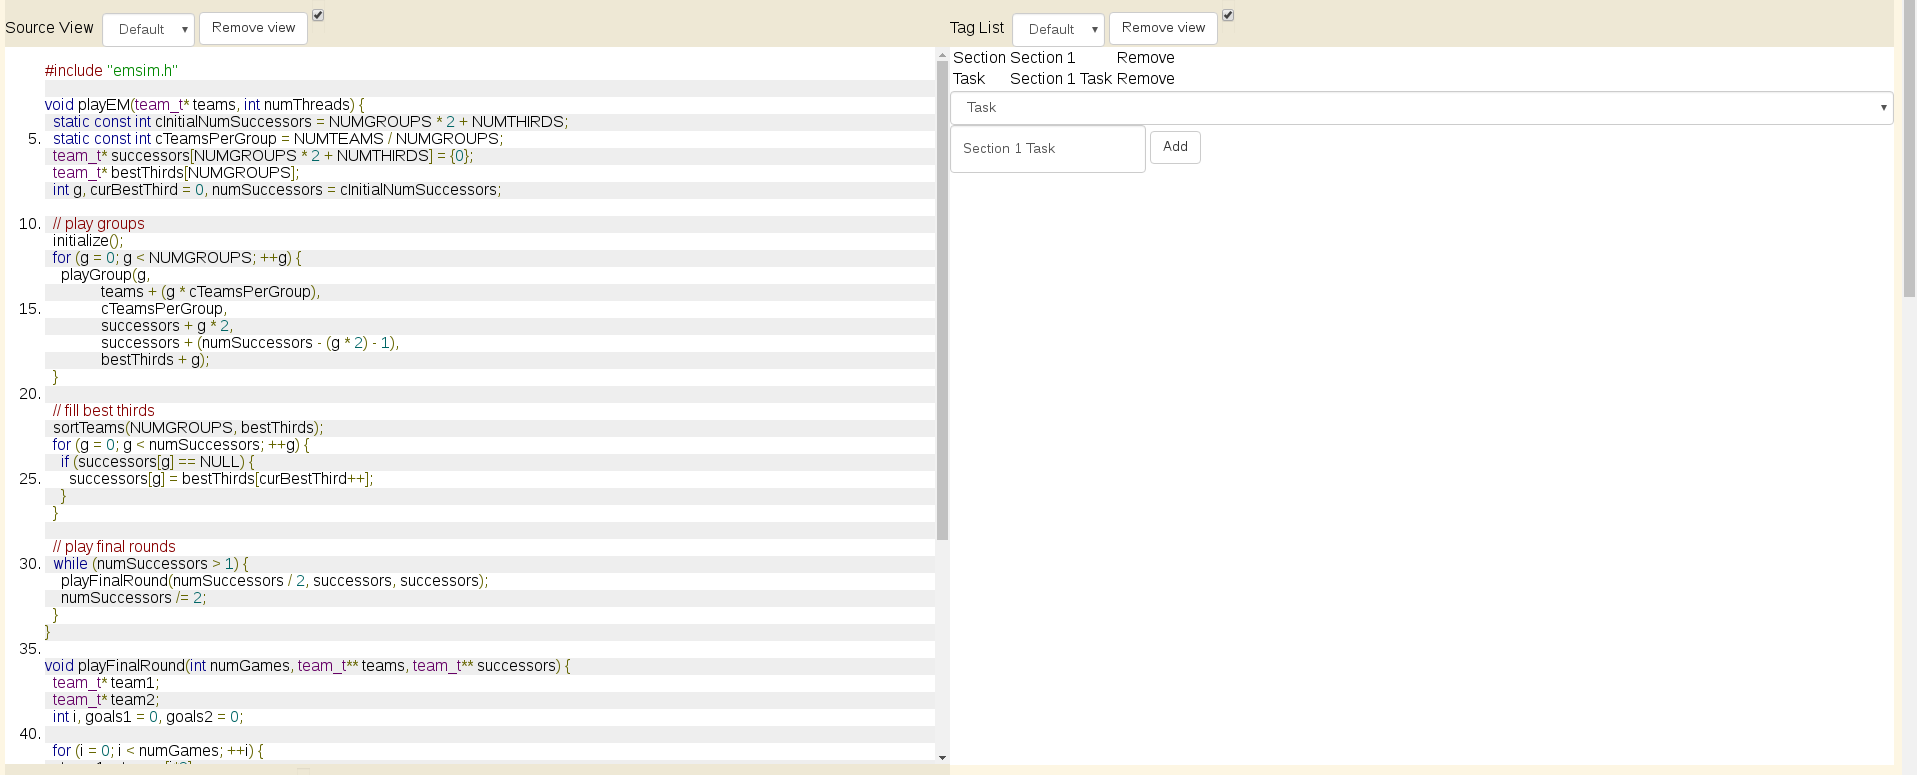
\includegraphics[width=0.8\textwidth]{tagging-view}
	\caption{UI for tagging}
	\label{cap1:tagview}
\end{figure}

\begin{figure}
	\begin{center}
		\begin{minted}{json}
{
  "tags": [
    { "name": "Section 1", "type": "Section" },
    { "name": "Section 1 Task", "type": "Task" }
  ],
  "tagInstructions": [
    { "tag": 1, "type": "Start", "location": 365 },
    { "tag": 1, "type": "Stop", "location": 372 },
    { "tag": 2, "type": "Start", "location": 367 }
  ]
}
		\end{minted}
	\end{center}
	\caption{Generated source.yaml}
	\label{cap1:source}
\end{figure}

\subsection {Dynamic analysis}

With \texttt{source.yaml} containing the tagging information it is possible to execute the dynamic analysis:

\begin{lstlisting}[style=BashInputStyle]
pin.sh -t libpintool\_dynamic.so -db emsim.db -filter filter.yaml \ 
  -source source.yaml -- emsim_seq em.db 1
\end{lstlisting}

The database from the static analysis is used for this execution and all the tracing and tag information is now stored within.

\subsection {Existing Visualizations}

The database must be imported again and all existing visualizations in \texttt{parceive-ui} continue to work as can be seen in Figure \ref{cap1:cct} and \ref{cap1:profiling}.

\begin{figure}[!ht]
	\centering
	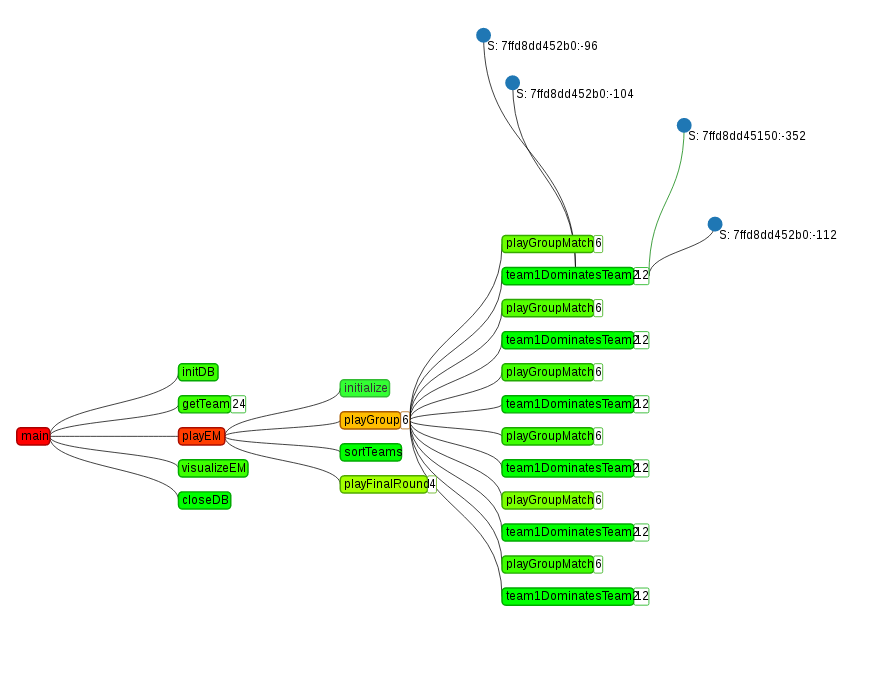
\includegraphics[width=0.8\textwidth]{cct}
	\caption{CCT View}
	\label{cap1:cct}
\end{figure}

\begin{figure}[!ht]
	\centering
	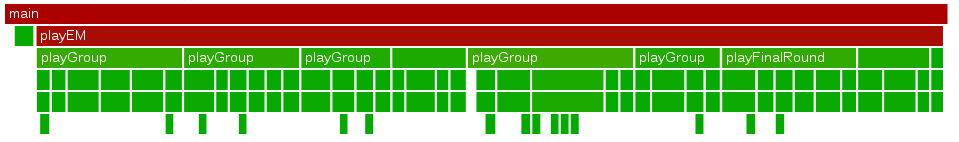
\includegraphics[width=0.8\textwidth]{profiling}
	\caption{Profiling View}
	\label{cap1:profiling}
\end{figure}

\subsection {Visualizations}

\section {Example}

To better illustrate how our tools are used we will analyze a simple application.

\subsection{The application}

Figure \ref{cap1:example:code} shows the code we will use for this example. The application allocates a memory reference and initializes  it using a constant value. We will simulate parallelization of the only loop in the application

\begin{figure}
	\begin{center}
		\inputminted[linenos]{c}{../tests/test4.c}
	\end{center}
	\caption{\texttt{test4.c} Simple test application}
	\label{cap1:example:code}
\end{figure}

\subsection{Static analysis}

The first step we will need to perform is the static analysis.

\begin{lstlisting}[style=BashInputStyle]
pin.sh -ifeellucky -t libpintool_static.so -db test4.db -- ./test4
\end{lstlisting}

After running the static analysis the Parceive UI can be used to navigate the source code of the application as can be seen in Figure \ref{cap1:example:code-view}. In the next section we will tag the code.

\begin{figure}[!ht]
	\centering
	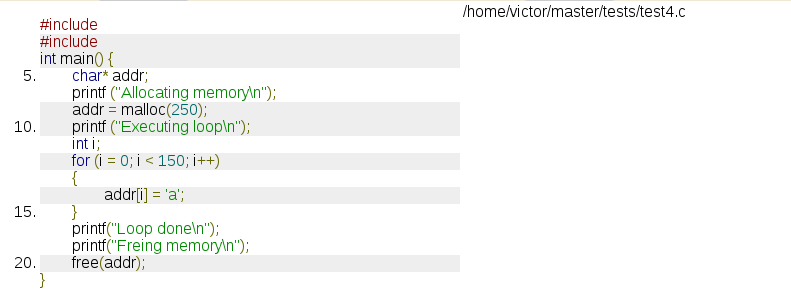
\includegraphics[width=1\textwidth]{simple-code}
	\caption{Source code view}
	\label{cap1:example:code-view}
\end{figure}

\subsection{Tagging the code}

Tagging the code is can be done by hand, but is much easier by using the UI. Figure \ref{cap1:example:code-tag} shows how Tags and TagInstructions can be created. For this example we add two tags:

\begin{itemize}
	\item A Section that wraps around the loop. It start on line 10 and stops on line 17.
	\item A Task Tag that marks the start of tasks inside the section.
\end{itemize}

\begin{figure}[!ht]
	\centering
	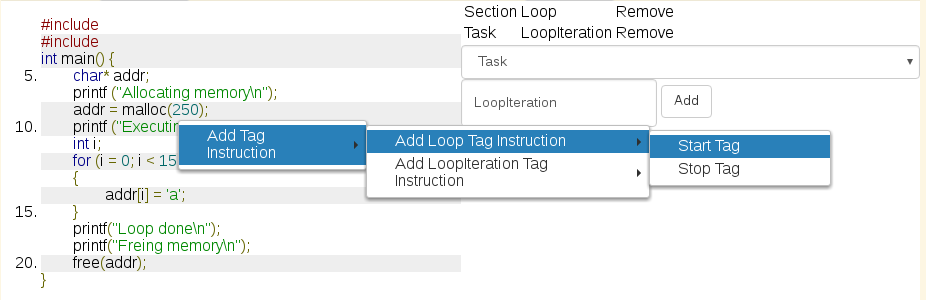
\includegraphics[width=1\textwidth]{simple-tag}
	\caption{Tagging view}
	\label{cap1:example:code-tag}
\end{figure}

After the tagging has been performed the UI generates the required input for the dynamic analysis as can be seen in Figure \ref{cap1:example:code-source}. This configuration is used by the dynamic analysis that will be performed in the next step.

\begin{figure}[!ht]
	\centering
	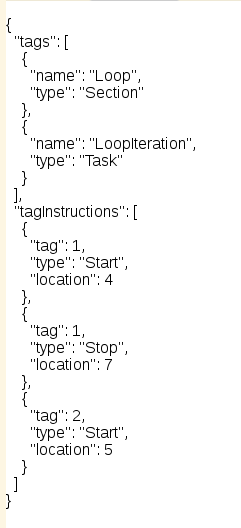
\includegraphics[width=0.3\textwidth]{simple-source}
	\caption{Tagging output}
	\label{cap1:example:code-source}
\end{figure}

\subsection{Dynamic analysis}

Now we will perform the dynamic analysis to obtain useful insight into the application:

\begin{lstlisting}[style=BashInputStyle]
pin.sh -ifeellucky -t libpintool_dynamic.so -db test4.db \
	-source source-test4.yaml -- ./test4
\end{lstlisting}

\begin{figure}[!ht]
	\centering
	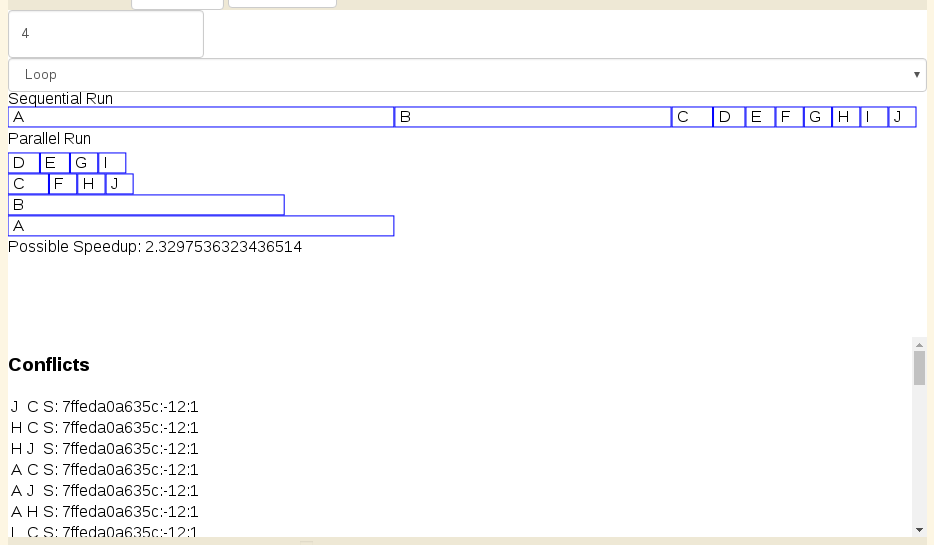
\includegraphics[width=0.9\textwidth]{simple-run1}
	\caption{Result after dynamic analysis}
	\label{cap1:example:code-run1}
\end{figure}

Figure \ref{cap1:example:code-run1} shows the Section view that presents the information obtained by the analysis. Using 4 cores and an ideal scheduling it is possible to speed up the \texttt{Loop} section by a factor of 2.32, but a large number of memory conflicts have been detected.

By using the Detail View that is part of Parceive we can see where the variable for each conflict is accessed. We can see that the update of \texttt{i} on each loop iteration conflicts with checking the condition and calculating the array index.

\subsection{Filtering conflicts}

The variable \texttt{i} is reported as a conflict between each task as it is read by the array access and written each loop iteration. This will not be an issue when parallelizing and we can also configure our tools to ignore it.

This is achieved by adding an ignore entry to the dynamic analysis as can be seen in Figure \ref{cap1:example:code-ignore}. The new execution illustrated in Figure \ref{cap1:example:code-run2} shows that there are no relevant conflicts can the loop could be parallelized.

After ignoring \texttt{i} we can see that each iteration of the loop accesses distinct memory locations so they can be executed in parallel without altering the behavior of the application. This particular example is trivial to analyze by hand, but our tool also scales to larger and more complex applications where performance benefits and dependencies can not be easily observed.

\begin{figure}
	\begin{center}
		\begin{minted}{yaml}
{
  "tags": [ ... ],
  "tagInstructions": [ ... ],
  "ignore": [
    {"function": 1, "delta": -12}
  ]
}
		\end{minted}
	\end{center}
	\caption{\texttt{source.yaml} update}
	\label{cap1:example:code-ignore}
\end{figure}

\begin{figure}[!ht]
	\centering
	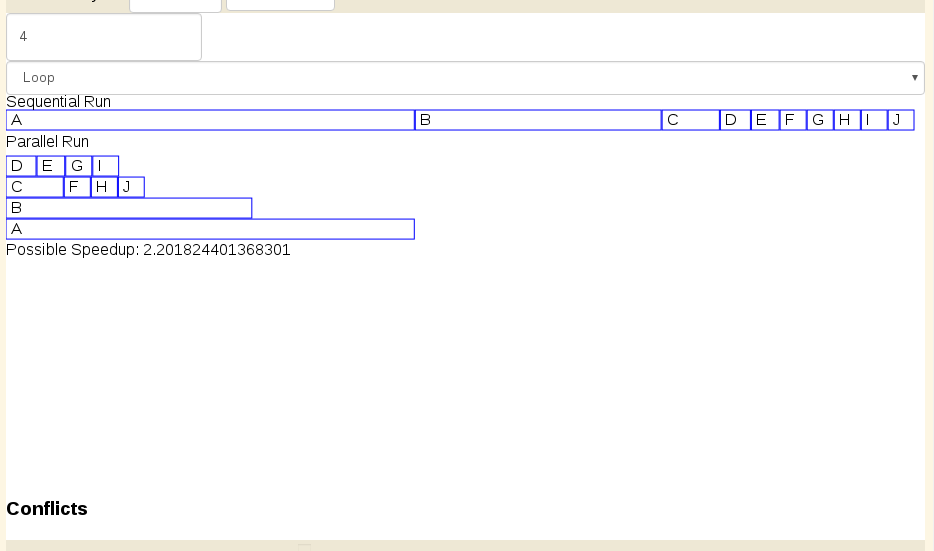
\includegraphics[width=0.9\textwidth]{simple-run2}
	\caption{Result after dynamic analysis with filtering}
	\label{cap1:example:code-run2}
\end{figure}

\section {Outline}

Chapter 2 provides an broad introduction into concepts and implementations that have made this thesis possible and worthwhile.

In chapter 3 we present the implementation of \texttt{pintool\_static.so}, \texttt{pintool\_dynamic.so} and visualizations that display data from specialized analyses. New analyses and visualizations can be easily developed.

Chapter 4 applies our tools to \texttt{emsim} \cite{parceive} and bzip \cite{bzip} compression of files. The first will show the utility of the section analysis and the latter of the pipeline analysis.

The last chapter contains our conclusion, comparisons to existing tools and possible future improvements that can be implemented for our tools.